\chapter{The Commander Calc Screen}
\label{ch:screen}

\ccprod{} uses the whole of an 80-column by 60-line text screen and draws every
character of it itself, straight into video memory. Nothing scrolls off the
top, nothing is printed, and there is no command line: the display is a single
fixed layout, and every one of its sixty lines has a job.

\index{screen!layout}
Figure~\ref{fig:screen} is the whole of it.

\begin{ccfigure}
\ccscreenscale{0.82}
\makebox[\linewidth]{%
\begin{tikzpicture}
\node[inner sep=0pt,anchor=north west] (scr) at (0,0) {%
\ccscreenbegin{80}{60}
  % --- row 0: the menu bar -------------------------------------------------
  \ccfillrow{0}{x16lgrey}
  \cctext{0}{1}{x16black}{File~~Edit~~Layout~~Data~~Chart~~Sheet}
  % --- row 1: the formula bar ----------------------------------------------
  \ccfill{1}{0}{11}{x16black}
  \ccfill{1}{12}{68}{x16black}
  \cctext{1}{1}{x16yellow}{B9}
  \cctext{1}{10}{x16yellow}{|}
  \cctext{1}{12}{x16yellow}{=SUM(B2:B7)}
  % --- row 2: the column headings ------------------------------------------
  \ccfillrow{2}{x16lgrey}
  \cccolhdr{2}{0}{A}{0}
  \cccolhdr{2}{1}{B}{1}
  \cccolhdr{2}{2}{C}{0}
  \cccolhdr{2}{3}{D}{0}
  \cccolhdr{2}{4}{E}{0}
  \cccolhdr{2}{5}{F}{0}
  \cccolhdr{2}{6}{G}{0}
  \cccolhdr{2}{7}{H}{0}
  % --- rows 3..56: the worksheet -------------------------------------------
  \foreach \r in {1,...,54}{\ccrowhdr{\the\numexpr\r+2\relax}{\r}{x16black}{x16lgrey}}
  \ccrowhdr{11}{9}{x16black}{x16yellow}

  % Headings are text, so they sit to the left of their columns while the
  % figures sit to the right. That is the program's own rule and the figure
  % shows it rather than tidying it away.
  \cccellL{3}{0}{x16black}{Category}
  \cccellL{3}{1}{x16black}{Jan}
  \cccellL{3}{2}{x16black}{Feb}
  \cccellL{3}{3}{x16black}{Mar}
  \cccellL{3}{4}{x16black}{Total}

  \cccellL{4}{0}{x16black}{Salaries}
  \cccellR{4}{1}{x16black}{\$8400.00}
  \cccellR{4}{2}{x16black}{\$8400.00}
  \cccellR{4}{3}{x16black}{\$8650.00}
  \cccellR{4}{4}{x16black}{\$25450.00}

  \cccellL{5}{0}{x16black}{Rent}
  \cccellR{5}{1}{x16black}{\$3000.00}
  \cccellR{5}{2}{x16black}{\$3000.00}
  \cccellR{5}{3}{x16black}{\$3000.00}
  \cccellR{5}{4}{x16black}{\$9000.00}

  \cccellL{6}{0}{x16black}{Power}
  \cccellR{6}{1}{x16black}{\$418.20}
  \cccellR{6}{2}{x16black}{\$377.65}
  \cccellR{6}{3}{x16black}{\$291.40}
  \cccellR{6}{4}{x16black}{\$1087.25}

  \cccellL{7}{0}{x16black}{Supplies}
  \cccellR{7}{1}{x16black}{\$226.00}
  \cccellR{7}{2}{x16black}{\$194.75}
  \cccellR{7}{3}{x16black}{\$310.05}
  \cccellR{7}{4}{x16black}{\$730.80}

  \cccellL{8}{0}{x16black}{Travel}
  \cccellR{8}{1}{x16black}{\$1140.00}
  \cccellR{8}{2}{x16black}{\$0.00}
  \cccellR{8}{3}{x16black}{\$865.50}
  \cccellR{8}{4}{x16black}{\$2005.50}

  \cccellL{9}{0}{x16black}{Insurance}
  \cccellR{9}{1}{x16black}{\$204.00}
  \cccellR{9}{2}{x16black}{\$204.00}
  \cccellR{9}{3}{x16black}{\$204.00}
  \cccellR{9}{4}{x16black}{\$612.00}

  \cccellL{11}{0}{x16black}{Total}
  \cccursor{11}{1}
  \cccellR{11}{1}{x16white}{\$13388.20}
  \cccellR{11}{2}{x16black}{\$12176.40}
  \cccellR{11}{3}{x16black}{\$13320.95}
  \cccellR{11}{4}{x16black}{\$38885.55}

  \cccellL{13}{0}{x16black}{Largest}
  \cccellR{13}{1}{x16black}{\$8400.00}
  \cccellL{14}{0}{x16black}{Average}
  \cccellR{14}{1}{x16black}{\$2231.37}

  % --- row 57: the worksheet tabs ------------------------------------------
  \ccfillrow{57}{x16lgrey}
  \ccfill{57}{0}{10}{x16yellow}
  \cctext{57}{1}{x16black}{Budget}
  \cctext{57}{11}{x16black}{Notes}
  \cctext{57}{22}{x16black}{BUDGET.X16S}
  % --- row 58: the status bar ----------------------------------------------
  \ccfillrow{58}{x16lgrey}
  \cctext{58}{1}{x16black}{READY}
  \cctext{58}{8}{x16black}{B9}
  \cctext{58}{18}{x16black}{516088~bytes~free}
  % --- row 59: the message line --------------------------------------------
\ccscreenend
};
% ---- callouts ------------------------------------------------------------
\begin{scope}[x=\ccchw,y=-\ccchh,shift={(scr.north west)}]
  \cccallout{Menu bar}{(82.5,-1.2)}{(72,0.5)}
  \cccallout{Formula bar}{(82.5,2.2)}{(76,1.5)}
  \cccallout{Column headings}{(82.5,5.6)}{(72,2.5)}
  \cccallout{Worksheet area}{(82.5,26)}{(66,26.5)}
  \cccallout{Worksheet tabs}{(82.5,53)}{(34,57.5)}
  \cccallout{Status line}{(82.5,58.5)}{(50,58.5)}
  \cccallout[east]{Row numbers}{(-2.5,20)}{(2.5,20.5)}
  \cccallout[east]{Cell cursor}{(-2.5,11.5)}{(16,11.5)}
\end{scope}
\end{tikzpicture}}
\caption{The \ccprod{} screen}
\label{fig:screen}
\end{ccfigure}

\section{What is on each line}

The layout is computed from the screen size at startup, so the line numbers
below are for the 80 by 60 display \ccprod{} asks for and normally gets. If the
machine is in a smaller text mode the program adapts, and it refuses to run at
all in anything shorter than ten lines.

\begin{cctable}{Line}{Contents}{0.72in}{4.1in}
0 & The menu bar, whether or not a menu is open. It always reads: \newline
\msg{~File~~Edit~~Layout~~Data~~Chart~~Sheet} \newline
with \msg{Commander Calc} at the right-hand end, which is a button --- see
\hyperref[sec:about]{The About box} below. \\
1 & The formula bar: the address of the current cell, a vertical bar, and what
that cell really contains. \\
2 & The column headings, \lit{A} through \lit{IV}. \\
3--56 & The worksheet: fifty-four rows of cells with their row numbers down the
left. \\
57 & The worksheet tabs, and after them the name of the workbook file. \\
58 & The status line. \\
59 & The message line. Blank almost always; the \menupath{Find} prompt and the
\menupath{Delete row} question are the only things that use it. \\
\end{cctable}

\section{The formula bar}
\index{formula bar}

The formula bar is the line that tells you the truth about a cell. The
worksheet shows you what a cell \emph{displays} --- rounded, formatted, and cut
off at the column edge. The formula bar shows you what it \emph{contains}.

\begin{ccfigure}
\ccscreenscale{1.5}
\begin{tikzpicture}
\node[inner sep=0pt,anchor=north west] (fb) at (0,0) {%
\ccscreenbegin{44}{1}
  \ccfill{0}{0}{11}{x16black}
  \ccfill{0}{12}{32}{x16black}
  \cctext{0}{1}{x16yellow}{B9}
  \cctext{0}{10}{x16yellow}{|}
  \cctext{0}{12}{x16yellow}{=SUM(B2:B7)}
\ccscreenend
};
\begin{scope}[x=\ccchw,y=-\ccchh,shift={(fb.north west)}]
  \draw[ccink,line width=0.4pt] (1,-0.9) -- (1,-0.2);
  \draw[ccink,line width=0.4pt] (10.5,-1.7) -- (10.5,-0.2);
  \draw[ccink,line width=0.4pt] (17,-0.9) -- (17,-0.2);
  \node[anchor=south west,font=\sffamily\fontsize{7.4}{8.6}\selectfont,
        inner sep=1pt] at (0.4,-0.9) {Cell address};
  \node[anchor=south west,font=\sffamily\fontsize{7.4}{8.6}\selectfont,
        inner sep=1pt] at (6.5,-1.7) {Separator};
  \node[anchor=south west,font=\sffamily\fontsize{7.4}{8.6}\selectfont,
        inner sep=1pt] at (16.4,-0.9) {Contents of the cell};
\end{scope}
\end{tikzpicture}
\caption{The formula bar, showing a formula cell}
\label{fig:formulabar}
\end{ccfigure}

The address occupies nine characters, which is exactly enough for \cellref{IV65535},
the last cell there is. After the separator come sixty-eight characters of cell
contents:

\begin{ccsteps}
\item For a formula, the formula as you wrote it --- \lit{=SUM(B2:B7)}, not
\lit{17388.2}.
\item For a number, the number unformatted. A cell displaying \lit{\$8.50} in
the worksheet shows \lit{8.5} here.
\item For text, the text.
\item For a blank cell, nothing.
\end{ccsteps}

While you are typing, the formula bar becomes the edit line: it shows what you
have typed so far, with one character highlighted to mark the insertion point.
If what you are typing is longer than sixty-eight characters, the line scrolls
horizontally to keep that point in view.

\begin{ccnote}
The formula bar is the only place a formula is ever visible. \ccprod{} has no
command that shows formulas in the worksheet in place of their results.
\end{ccnote}

\section{The status line}
\index{status line}\index{mode indicator}

\begin{ccfigure}
\ccscreenscale{1.5}
\begin{tikzpicture}
\node[inner sep=0pt,anchor=north west] (sb) at (0,0) {%
\ccscreenbegin{44}{1}
  \ccfillrow{0}{x16lgrey}
  \cctext{0}{1}{x16black}{READY}
  \cctext{0}{8}{x16black}{B9}
  \cctext{0}{18}{x16black}{516088~bytes~free}
\ccscreenend
};
\begin{scope}[x=\ccchw,y=-\ccchh,shift={(sb.north west)}]
  \draw[ccink,line width=0.4pt] (2,-0.9) -- (2,-0.2);
  \draw[ccink,line width=0.4pt] (9,-1.7) -- (9,-0.2);
  \draw[ccink,line width=0.4pt] (24,-0.9) -- (24,-0.2);
  \node[anchor=south west,font=\sffamily\fontsize{7.4}{8.6}\selectfont,
        inner sep=1pt] at (1.4,-0.9) {Mode};
  \node[anchor=south west,font=\sffamily\fontsize{7.4}{8.6}\selectfont,
        inner sep=1pt] at (6.6,-1.7) {Current cell};
  \node[anchor=south west,font=\sffamily\fontsize{7.4}{8.6}\selectfont,
        inner sep=1pt] at (23.4,-0.9) {Free memory};
\end{scope}
\end{tikzpicture}
\caption{The status line}
\label{fig:statusline}
\end{ccfigure}

\subsection{The mode indicator}

Five characters at the left of the status line, and there are exactly three
things they can say.

\begin{cctable}{Indicator}{Meaning}{0.8in}{4.02in}
\msg{READY} & \ccprod{} is waiting for you. Nothing has been changed since the
workbook was last saved or opened. \\
\msg{MODIF} & The same, except that the workbook has been modified. Leaving the
program, opening another workbook or starting a new one will ask you to confirm
first. \\
\msg{EDIT} & You are typing into a cell. The formula bar is showing what you
have typed, not what the cell contains. \\
\end{cctable}

\msg{MODIF} appears the moment anything is changed and stays until the workbook
is saved, opened or replaced. It is the only warning you get that there is work
in memory which is not on the card.

\subsection{The current cell}

Eight characters giving the address of the cell the cursor is on --- the same
address as in the formula bar, repeated at the other end of the screen so that
it is near whichever end you happen to be looking at.

\subsection{The free memory readout}
\index{memory!free readout}

The rest of the status line is a count of free banked RAM, as a plain decimal
number followed by \msg{bytes free}. On a machine with the standard 512K you
will see about half a million; on a fully expanded 2M machine, about two
million.

\begin{ccnote}
This figure is measured once, when the program starts, and is never updated.
It tells you how large a workbook the machine can hold. It does not tell you
how much of it you have used.
\end{ccnote}

One other thing can appear in this field. If the C stack ever overflows,
\ccprod{} replaces the whole status text with \msg{STACK!}. See
Chapter~\ref{ch:messages}.

\subsection{The recalculation indicator}
\index{status line!CALC}

The last few characters of the status line are empty almost always. One word can
appear there:

\begin{cctable}{Indicator}{Meaning}{0.8in}{4.02in}
\msg{CALC} & \textbf{The answers on screen are stale.} Automatic recalculation
has been switched off and something has changed since the last one. \\
\end{cctable}

Nothing is shown at any other time --- not while automatic recalculation is on,
and not while it is off but everything is up to date. The indicator marks the
one state worth interrupting you about. Chapter~\ref{ch:recalc} explains the
switch.

\section{The worksheet area}
\index{worksheet!area}

Fifty-four rows of cells, with a six-character gutter down the left holding the
row numbers, and columns ten characters wide unless a workbook file says
otherwise. That gives seven whole columns on screen and a four-character sliver
of the eighth.

\subsection{The cell cursor}
\index{cell cursor}

The cell the cursor is on is drawn in reverse video --- white on black --- for
the full width of its column. At the same time its row number and its column
heading are highlighted in yellow, which is what lets you find the cursor at a
glance in a screen full of numbers.

\subsection{How values are placed in a cell}

A value is drawn inside its own column and nowhere else.

\begin{ccsteps}
\item Numbers, and cells holding dates, are set to the right of the column.
\item Text, \msg{TRUE} and \msg{FALSE}, and error values are set to the left.
\item A formula is aligned by what it produced, not by the fact that it is a
formula: a formula returning a number goes right, one returning text goes left.
\item A workbook that came from a file may carry an explicit left or right
alignment for a cell, which overrides all of the above.
\end{ccsteps}

\begin{cccaution}
A value too wide for its column is cut off at the column edge. It is not
spilled into the empty cell next door, and there is no \lit{\#\#\#\#} marker to
tell you it happened --- what you see is a shortened number that still looks
like a number. If a column of figures looks wrong, check the formula bar before
you check the arithmetic. Column widths cannot be changed from the keyboard;
see Chapter~\ref{ch:formats}.
\end{cccaution}

\section{The worksheet tabs}
\index{worksheet!tabs}

Line 57 carries one tab per worksheet, ten characters each, with the active one
highlighted in yellow. A worksheet name may be up to thirty-one characters
long, but only the first nine of them fit on a tab.

After the last tab, if there is room left on the line, \ccprod{} prints the name
of the workbook file. A workbook that has never been saved has no name there.

\section{Colours}

\ccprod{} uses eight of the Commander X16's sixteen colours, and always the
same eight for the same purposes.

\begin{cctable}{Area}{Colour}{1.55in}{3.27in}
Worksheet cells & Black on white \\
Cell cursor & White on black \\
Row and column headings & Black on light grey \\
Heading of the cursor's row and column & Black on yellow \\
Menu bar, tabs, status line & Black on light grey \\
Open menu title, highlighted menu item & Black on yellow \\
Menu items & White on medium grey \\
Formula bar & Yellow on black \\
Dialogue box body & Black on light grey \\
Dialogue title bar, buttons, selected row & White on blue \\
\end{cctable}

None of these can be changed.

\section{The About box}
\label{sec:about}
\index{About box}\index{version number}

\textbf{Click \msg{Commander Calc} at the right-hand end of the menu bar.} A box
opens in the middle of the screen naming the program and the version this copy
was built as:

\begin{ccfigure}
\ccscreenscale{1.3}
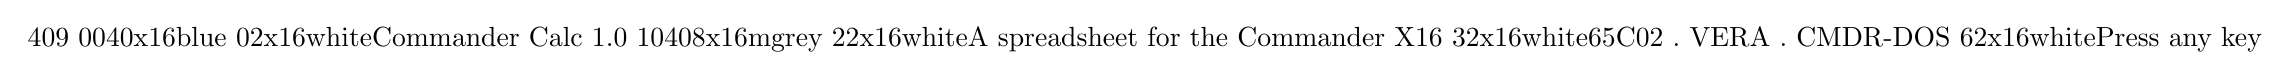
\begin{tikzpicture}
\node[inner sep=0pt,anchor=north west] (ab) at (0,0) {%
\ccscreenbegin{40}{9}
  \ccfill{0}{0}{40}{x16blue}
  \cctext{0}{2}{x16white}{Commander~Calc~1.0}
  \ccfillbox{1}{0}{40}{8}{x16mgrey}
  \cctext{2}{2}{x16white}{A~spreadsheet~for~the~Commander~X16}
  \cctext{3}{2}{x16white}{65C02~.~VERA~.~CMDR-DOS}
  \cctext{6}{2}{x16white}{Press~any~key}
\ccscreenend
};
\end{tikzpicture}
\caption{The About box}
\label{fig:about}
\end{ccfigure}

Any key closes it. It is the one part of \ccprod{} that can only be reached with
the mouse --- there is no menu entry and no keyboard shortcut.

\begin{ccnote}
The version shown is fixed when the program is built, so it is the reliable way
to tell one copy from another. If you are reporting something odd, this is the
number to quote.
\end{ccnote}
